\index{MMS} \index{method of manufactured solutions}

The method of manufactured solutions is a relatively simple way of carrying out
code verification. In essence, one postulates a solution for the PDE at hand (as
well as the proper boundary conditions), inserts it in the PDE and computes the 
corresponding source term. 
The same source term and boundary conditions will then be used in a numerical 
simulation so that the computed solution can be compared with the (postulated)
true analytical solution. 

Examples of this approach are to be found in \cite{dohu03,busa13,bodg06}.


%-----------------------------------------------------------------------------
\subsubsection{Analytical benchmark I \label{mms1} - "DH"}

Taken from \cite{dohu03}. We consider a two-dimensional problem 
in the square domain $\Omega=[0,1]\times[0,1]$, which possesses a closed-form analytical 
solution. The problem consists of determining the velocity field ${\vec \upnu} = (u,v)$ 
and the pressure $p$ such that 
\begin{eqnarray}
\eta \Delta {\vec \upnu} - {\vec \nabla} p + {\vec b} &=& \vec 0 \quad\quad {\rm in} \; \Omega\\
\vec{\nabla} \cdot \vec{v} &=& 0 \quad\quad {\rm in} \; \Omega\\
\vec{v}&=&\vec{0} \quad\quad {\rm on} \; \Gamma_D
\end{eqnarray}
where the fluid viscosity is taken as $\eta=1$.
The components of the body force $\vec{b}$ are prescribed as 
\begin{eqnarray}
b_x &=& (12 - 24y) x^4 + (-24 + 48y) x^3 + (-48y + 72y^2 - 48 y^3 + 12) x^2 \nonumber\\
    && + (-2 + 24y -72y^2+48y^3)x + 1-4y + 12y^2-8y^3 \nonumber\\ 
b_y &=& (8 - 48y + 48 y^2) x^3 + (-12 + 72y - 72y^2) x^2  \nonumber\\
    && + (4 - 24y + 48y^2 - 48y^3 + 24y^4) x - 12y^2 + 24y^3 - 12y^4  \nonumber
\end{eqnarray}
With this prescribed body force, the exact solution is 
\begin{eqnarray}
u(x,y) &=& x^2(1- x)^2 (2y - 6y^2 + 4y^3)  \nonumber\\
v(x,y) &=& -y^2 (1 - y)^2 (2x - 6x^2 + 4x^3) \nonumber\\
p(x,y) &=& x(1 -x)- 1/6 \nonumber 
\end{eqnarray}
Note that the pressure obeys $\int_{\Omega} p \; d\Omega = 0$.
One can turn to the spatial derivatives of the fields:
\begin{eqnarray}
\dot{\varepsilon}_{xx}=\frac{\partial u}{\partial x} &=&  (2x -6x^2 +4 x^3 ) (2y - 6y^2 + 4y^3)  \\
\dot{\varepsilon}_{yy}=\frac{\partial v}{\partial y} &=&  - (2x -6x^2 +4 x^3 ) (2y - 6y^2 + 4y^3)  \\
\dot{\varepsilon}_{xy}=\frac{1}{2}\left(\frac{\partial u}{\partial y}+\frac{\partial v}{\partial x}\right) 
&=&=\frac{1}{2}\left( x^2(1- x)^2 ( 2-12y+12y^2  ) -y^2 (1-y)^2 (2-12x+12x^2) \right)
\end{eqnarray}
with of course  ${\vec \nabla} \cdot {\vec \upnu} = 0$ and 
\begin{eqnarray}
\frac{\partial p}{\partial x} &=& 1-2x  \\
\frac{\partial p}{\partial y} &=& 0
\end{eqnarray}

The velocity and pressure fields look like:

\begin{center}
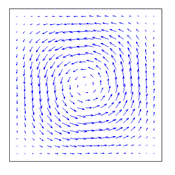
\includegraphics[height=4cm]{images/mms/Ex1_Q2Q1_velo.png}
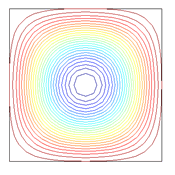
\includegraphics[height=4cm]{images/mms/Ex1_Q2Q1_streamlines.png}
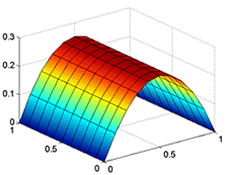
\includegraphics[height=4cm]{images/mms/Ex1_Q2Q1_pres.png}\\
{\small http://ww2.lacan.upc.edu/huerta/exercises/Incompressible/Incompressible\_Ex1.htm}
\end{center}

As shown in \cite{dohu03}, If the LBB condition is not satisfied, spurious oscillations spoil the pressure approximation. 
Figures below show results obtained with a mesh of 20x20 Q1P0 (left) and P1P1 (right) elements:
\begin{center}
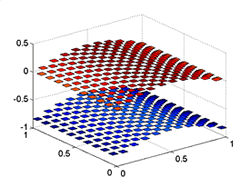
\includegraphics[height=5cm]{images/mms/Ex1_Q1P0_pres.png}
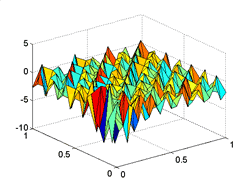
\includegraphics[height=5cm]{images/mms/Ex1_P1P1_pres.png}]]
{\small http://ww2.lacan.upc.edu/huerta/exercises/Incompressible/Incompressible\_Ex1.htm}
\end{center}

Taking into account that the proposed problem has got analytical solution, it is easy to analyze convergence of the different pairs of elements:
\begin{center}
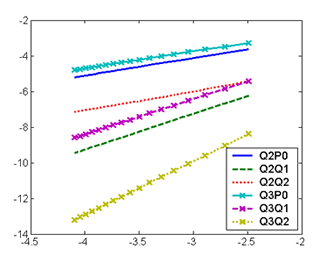
\includegraphics[height=7cm]{images/mms/Ex1_conv_qua.png}\\
{\small http://ww2.lacan.upc.edu/huerta/exercises/Incompressible/Incompressible\_Ex1.htm}
\end{center}

One can also compute the stress components:
\begin{eqnarray}
\sigma_{xx} &=&  2x^2(2x - 2)(4y^3 - 6y^2 + 2y) + 4x(-x + 1)^2*(4y^3 - 6y^2 + 2y) - x(-x + 1) + 1/6 \\
\sigma_{xy} &=&  x^2(-x + 1)^2*(12y^2 - 12y + 2) - y^2(-y + 1)^2*(12x^2 - 12x + 2) \\
\sigma_{yy} &=&  -x(-x + 1) - 2y^2(2y - 2)(4x^3 - 6x^2 + 2x) - 4y(-y + 1)^2(4x^3 - 6x^2 + 2x) + 1/6
\end{eqnarray}


All the necessary functions to do this benchmark are in {\tt mms/dh.py}:
\lstinputlisting[language=python]{mms/dh.py}


%-----------------------------------------------------------------------------
\subsubsection{Analytical benchmark II \label{mms2} - "DB2D"}

Taken from \cite{dobo04,bodg06}. It is for a unit square with $\nu=\mu/\rho=1$ and the smooth exact solution is
\begin{eqnarray}
u(x,y) &=& x+x^2 - 2xy+x^3 - 3xy^2 + x^2y \\
v(x,y) &=& -y-2xy+y^2 -3x^2y + y^3 - xy^2 \\
p(x,y) &=& xy+x+y+x^3y^2 - 4/3
\end{eqnarray}
Note that the pressure obeys $\int_{\Omega} p \; d\Omega = 0$

\begin{eqnarray}
b_x &=& - (1+y-3x^2y^2) \\
b_y &=& - (1-3x-2x^3y) 
\end{eqnarray}

This benchmark is also used in \cite{wosp14}.

%-----------------------------------------------------------------------------
\subsubsection{Analytical benchmark III \label{mms3} - "DB3D"}

This benchmark begins by postulating a polynomial solution 
to the 3D Stokes equation \cite{dobo04}:
\begin{equation}
{\bm v}
=
\left(
\begin{array}{c}
x+x^2+xy+x^3y \\
y + xy + y^2 + x^2 y^2\\
-2z - 3xz - 3yz - 5x^2 yz
\end{array}
\right)
\label{eqbur}
\end{equation}
and
\begin{equation}
p = xyz + x^3 y^3z - 5/32
\end{equation}
While it is then trivial to verify that this velocity field is divergence-free,  
the corresponding body force of the Stokes equation can be computed by  
inserting this solution into the momentum equation with a given viscosity $\mu$
(constant or position/velocity/strain rate dependent). 
The domain is a unit cube and velocity boundary conditions 
simply use Eq. (\ref{eqbur}). 
Note that the pressure fulfills 
\[
\int_\Omega p({\vec r}) d\Omega = 0.  
\]


\paragraph{Constant viscosity}
In this case, the right hand side writes:
\begin{eqnarray}
{\bm f} &=& 
-{\bm \nabla p} + 
\mu
\left(
\begin{array}{c}
2+6xy \\
2+2x^2+2y^2 \\
-10yz
\end{array}
\right) \nonumber\\
&=&
-
\left(
\begin{array}{c}
yz+3x^2 y^3z \\
xz+3 x^3 y^2 z \\
xy+x^3y^3
\end{array}
\right) 
+
\mu
\left(
\begin{array}{c}
2+6xy \\
2+2x^2+2y^2 \\
-10yz
\end{array}
\right)
\nonumber
\end{eqnarray}

We can compute the components of the strainrate tensor:
\begin{eqnarray}
\dot{\varepsilon}_{xx} &=& 1+2x+y+3x^2y\\
\dot{\varepsilon}_{yy} &=& 1+x+2y+2x^2y\\
\dot{\varepsilon}_{zz} &=& -2-3x-3y-5x^2y\\ 
\dot{\varepsilon}_{xy} &=&  \frac{1}{2} (x+y+2xy^2+x^3)\\
\dot{\varepsilon}_{xz} &=&  \frac{1}{2} (-3z-10xyz  )\\
\dot{\varepsilon}_{yz} &=&  \frac{1}{2} ( -3z -5x^2z )
\end{eqnarray}
Note that we of course have $\dot{\varepsilon}_{xx} +\dot{\varepsilon}_{yy} 
+\dot{\varepsilon}_{zz} =0$.

\paragraph{Variable viscosity}

In this case, the right hand side is obtained through
\begin{eqnarray}
{\bm f} &=& -{\bm \nabla p} + 
\mu
\left(
\begin{array}{c}
2+6xy \\
2+2x^2+2y^2 \\
-10yz
\end{array}
\right) \nonumber\\
&+&
\left(
\begin{array}{c}
2 \dot{\varepsilon}_{xx} \\
2 \dot{\varepsilon}_{xy} \\
2 \dot{\varepsilon}_{xz}
\end{array}
\right) \frac{\partial \mu}{\partial x}
+
\left(
\begin{array}{c}
2 \dot{\varepsilon}_{xy} \\
2 \dot{\varepsilon}_{yy} \\
2 \dot{\varepsilon}_{yz}
\end{array}
\right) \frac{\partial \mu}{\partial y}
+
\left(
\begin{array}{c}
2 \dot{\varepsilon}_{xz} \\
2 \dot{\varepsilon}_{yz} \\
2 \dot{\varepsilon}_{zz} 
\end{array}
\right) \frac{\partial \mu}{\partial z}
\end{eqnarray}


The viscosity can be chosen to be a smooth varying function:
\begin{equation}
\mu = exp(1 - \beta(x(1 - x) + y(1 - y) + z(1 - z)))
\end{equation}
Choosing $\beta=0$ yields a constant velocity $\mu=e^1$ (and greatly simplifies the right-hand side).
One can easily show that the ratio of viscosities $\mu^\star$
in the system follows $\mu^\star=\exp(-3\beta/4)$ so that choosing $\beta=10$ yields
$\mu^\star\simeq 1808$ and $\beta=20$ yields $\mu^\star\simeq 3.269\times10^6$.
In this case
\begin{eqnarray}
\frac{\partial \mu}{\partial x}&=&-4\beta(1-2x)\mu(x,y,z)\\
\frac{\partial \mu}{\partial y}&=&-4\beta(1-2y)\mu(x,y,z)\\
\frac{\partial \mu}{\partial z}&=&-4\beta(1-2z)\mu(x,y,z)
\end{eqnarray}


\cite{busa13} has carried out this benchmark for $\beta=4$, i.e.: 
\[
\mu(x,y,z)=\exp ( 1-4( x(1-x)+y(1-y)+z(1-z)  )  )
\]
In a unit cube, this yields a variable viscosity such that
$0.1353 < \mu <   2.7182$, i.e. a ratio of approx. 20 within the domain. We then have:
\begin{eqnarray}
\frac{\partial \mu}{\partial x}&=&-4(1-2x)\mu(x,y,z)\\
\frac{\partial \mu}{\partial y}&=&-4(1-2y)\mu(x,y,z)\\
\frac{\partial \mu}{\partial z}&=&-4(1-2z)\mu(x,y,z)
\end{eqnarray}

\todo[inline]{sort out mess wrt Eq 26 of busa13}


%-----------------------------------------------------------------------------
\subsubsection{Analytical benchmark IV \label{mms4} - "Bercovier \& Engelman"}

From \cite{been79}. The two-dimensional domain is a unit square. The body forces are:
\begin{eqnarray}
f_x &=& 128[ x^2(x-1)^2 12 (2y-1) + 2 (y-1)(2y-1)y(12x^2-12x+2)  ] \nn\\
f_y &=& 128[ y^2(y-1)^2 12 (2x-1) + 2 (x-1)(2x-1)y(12y^2-12y+2)  ] \nn\\
\end{eqnarray}
The solution is
\begin{eqnarray}
u &=& -256x^2(x-1)^2y(y-1)(2y-1) \nn\\
v &=&  256x^2(y-1)^2x(x-1)(2x-1) \nn\\
p &=& 0 
%p &=& (x-1/2)(y-1/2) 
\end{eqnarray}

Another choice:
\begin{eqnarray}
f_x &=& 128[ x^2(x-1)^2 12 (2y-1) + 2 (y-1)(2y-1)y(12x^2-12x+2)  ] + y - 1/2 \nn\\
f_y &=& 128[ y^2(y-1)^2 12 (2x-1) + 2 (x-1)(2x-1)y(12y^2-12y+2)  ] + x - 1/2 \nn\\
\end{eqnarray}
The solution is
\begin{eqnarray}
u &=& -256x^2(x-1)^2y(y-1)(2y-1) \nn\\
v &=&  256x^2(y-1)^2x(x-1)(2x-1) \nn\\
p &=& (x-1/2)(y-1/2) 
\end{eqnarray}


%-----------------------------------------------------------------------------
\subsubsection{Analytical benchmark V \label{mms5} - "VJ1"}

This is taken from Appendix D1 of \cite{john16}.

The domain $\Omega$ is a unit square. We consider the stream function
\[
\phi(x,y)=1000x^2(1-x)^4y^3(1-y)^2
\]
The velocity field is defined by
\begin{eqnarray}
u(x,y) &=&  \partial_y \phi = 1000(x^2(1-x)^4 y^2 (1-y)(3-5y)  ) \\
v(x,y) &=& -\partial_x \phi = 1000(-2x(1-x)^3(1-3x)y^3(1-y)^2)
\end{eqnarray}
and it is easy to verify that $\vec\nabla\cdot\vec v=0$.

The pressure is given by:
\[
p(x,y)=\pi^2( xy^3\cos(2\pi x^2y) - x^2y \sin(2\pi xy)) + \frac{1}{8}
\]

\begin{center}
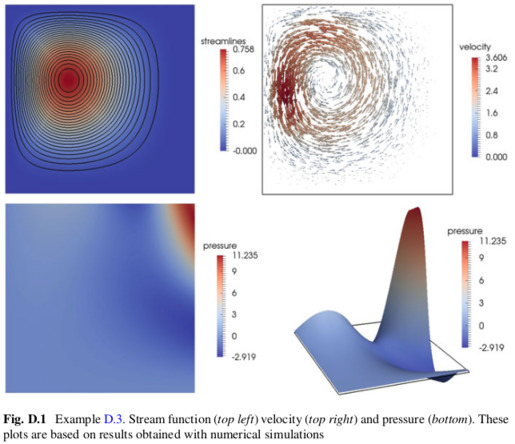
\includegraphics[width=8cm]{images/mms/mms5}\\
Taken from \cite{john16}.
\end{center}

\bscthesis \index{BSc Thesis}

%-----------------------------------------------------------------------------
\subsubsection{Analytical benchmark VI \label{mms6} - "Ilinca \& Pelletier"}
\index{Poiseuille flow} \index{Shear Heating}

This is taken from \cite{ilpe07}.

Let us consider the Poiseuille flow of a Newtonian fluid. The channel has 
isothermal flat walls located at $y=\pm h$. The velocity distribution is parabolic:
\[
u = u_0 \left(1-\frac{y^2}{h^2} \right) 
\quad\quad\quad
v=0
\]
where $u_0$ is the maximum velocity. The (steady state) temperature field is the solution of
the advection-diffusion equation:
\[
\rho C_p \vec v \cdot \vec\nabla T
= k \Delta T + \Phi
\]
where $\Phi$ is the dissipation function given by
\[
\Phi
=\eta \left[  
2\left(\frac{\partial u}{\partial x} \right)^2 + 
2\left(\frac{\partial v}{\partial y} \right)^2 +
\left( \frac{\partial v}{\partial x} + \frac{\partial u}{\partial y} \right)^2
\right]
=
\eta \left( \frac{\partial u}{\partial y} \right)^2 = 4 \eta \frac{u_0^2 y^2}{h^4}
\]
We logically assume that $T=T(y)$ so that $\partial T/\partial x=0$ and $\vec v \cdot \vec\nabla T=0$.
We then have to solve:
\[
k \frac{\partial^2 T}{\partial y^2} + 4 \eta \frac{u_0^2 y^2}{h^4} = 0
\]
We can integrate twice and use the boundary conditions $T(y=\pm h)=T_0$ to arrive at:
\[
T(y) = T_0 + \frac{1}{3} \frac{\eta u_0^2}{k} \left[ 1-\left(\frac{y}{h}\right)^4  \right]
\]
with a maximum temperature
\[
T_M = T(y=0) = T_0 + \frac{1}{3} \frac{\eta u_0^2}{k} 
\]

%-----------------------------------------------------------------------------
\subsubsection{Analytical benchmark VII \label{mms7} - "grooves"}

This benchmark was designed by Dave May. 
The velocity and pressure fields are given by
\begin{eqnarray}
u(x,y) &=& x^3 y + x^2 + xy + x \nn\\
v(x,y) &=& -\frac{3}{2}x^2y^2 - 2xy - \frac{1}{2}y^2 - y \nn\\
p(x,y) &=& x^2y^2 + xy + 5 + p_0
\end{eqnarray}
where $p_0$ is a constant to be determined based on the type of pressure normalisation.
The viscosity is chosen to be
\begin{equation}
\eta(x,y)=-\sin(p)+1+\epsilon = -\sin (x^2y^2 + xy + 5) + 1 + \epsilon 
\end{equation}
where $\epsilon$ actually controls the viscosity contrast. Note that inserting the polynomial 
expression of the pressure inside the viscosity expression makes the problem linear. 
We have
\begin{eqnarray}
\dot{\varepsilon}_{xx} = \frac{\partial u}{\partial x} &=& 3x^2y+2x+y+1 \nn\\
\dot{\varepsilon}_{yy} = \frac{\partial v}{\partial y} &=& -3x^2y-2x-y-1 \nn\\
\dot{\varepsilon}_{xy} = \frac{1}{2}\left(\frac{\partial u}{\partial y} + \frac{\partial v}{\partial x} \right)
&=& \frac{1}{2}\left(x^3+x-3xy^2-2y \right)
\end{eqnarray}
and we can verify that the velocity field is incompressible since ${\vec \nabla}\cdot{\vec \upnu} = 
\dot{\varepsilon}_{xx} + \dot{\varepsilon}_{yy} =0$.
The pressure gradient is given by
\begin{eqnarray}
\frac{\partial p}{\partial x} &=& 2xy^2+y \nn\\
\frac{\partial p}{\partial y} &=& 2x^2y+x \nn
\end{eqnarray}
The right hand side term of the Stokes equation is such that
\begin{eqnarray}
 - \frac{\partial p}{\partial x} + \frac{\partial s_{xx}}{\partial x} + \frac{\partial s_{yx}}{\partial y} +f_x&=&0\nn\\
 - \frac{\partial p}{\partial y} + \frac{\partial s_{xy}}{\partial x} + \frac{\partial s_{yy}}{\partial y} +f_y&=&0
\end{eqnarray}
with 
\begin{eqnarray}
\frac{\partial s_{xx}}{\partial x} 
&=& \frac{\partial (2 \eta \dot{\varepsilon}_{xx}) }{\partial x} = 2 \eta \frac{\partial  \dot{\varepsilon}_{xx} }{\partial x} +  2\frac{\partial \eta }{\partial x} \dot{\varepsilon}_{xx} \nn\\
\frac{\partial s_{zx}}{\partial z} 
&=& \frac{\partial (2 \eta \dot{\varepsilon}_{zx}) }{\partial z} = 2 \eta \frac{\partial  \dot{\varepsilon}_{zx} }{\partial z} +  2\frac{\partial \eta }{\partial z} \dot{\varepsilon}_{zx} \nn\\
\frac{\partial s_{xz}}{\partial x} 
&=& \frac{\partial (2 \eta \dot{\varepsilon}_{xz}) }{\partial x} = 2 \eta \frac{\partial  \dot{\varepsilon}_{xz} }{\partial x} +  2\frac{\partial \eta }{\partial x} \dot{\varepsilon}_{xz} \nn\\
\frac{\partial s_{zz}}{\partial z} 
&=& \frac{\partial (2 \eta \dot{\varepsilon}_{zz}) }{\partial z} = 2 \eta \frac{\partial  \dot{\varepsilon}_{zz} }{\partial z} +  2\frac{\partial \eta }{\partial z} \dot{\varepsilon}_{zz} \nn\\
\frac{\partial \eta }{\partial x} &=& -z (2 x z + 1) \cos(x^2 z^2 + x z + 5) \nn\\
\frac{\partial \eta }{\partial z} &=& -x (2 x z + 1) \cos(x^2 z^2 + x z + 5) \nn\\
\frac{\partial  \dot{\varepsilon}_{xx} }{\partial x} &=& 6xz+2 \nn\\
\frac{\partial  \dot{\varepsilon}_{zx} }{\partial z} &=& -3xz-1  \nn\\
\frac{\partial  \dot{\varepsilon}_{xz} }{\partial x} &=& \frac{1}{2}(3x^2+1-3z^2)  \nn\\
\frac{\partial  \dot{\varepsilon}_{zz} }{\partial z} &=& -3x^2-1  \nn
\end{eqnarray}

\index{pressure nullspace}
Velocity boundary conditions are prescribed on all four boundaries so that the pressure is known up to a constant
(the pressure solution has a nullspace), 
and the $p_0$ constant can be determined by requiring that
\[
\int_0^L\int_0^L p(x,y) \; dx dy = 
\int_0^L\int_0^L (x^2y^2+xy+5) dx dy + \int_0^L \int_0^L p_0 \; dxdy = 
\int_0^L\int_0^L (x^2y^2+xy+5) dx dy + p_0 L^2 =0 
\]
where $L$ is the size of the square domain.
Then
\[
p_0 =-  \frac{1}{L^2}  \int_0^L\int_0^L (x^2y^2+xy+5) dx dy
= -\frac{L^4}{9}-\frac{L^2}{4} - 5 
\]
\[
\]
%\begin{itemize}
%\item
%When the domain is $1\times 1$, $p_0=-\frac{1}{9}-\frac{1}{4} - 5 = -193/36$.
%\item
%When the domain is $2\times 2$, $p_0=-\frac{16}{9}-\frac{4}{4} - 5*4 = -70/9$.
%\item
%When the domain is $3\times 3$, $p_0=-\frac{81}{9}-\frac{9}{4} - 5*9 = -585/16$.
%\item
%When the domain is $4\times 4$, $p_0=-\frac{256}{9}-\frac{16}{4} - 5*16 = -1348/9$.
%\end{itemize}

As seen in the following figure, the value of $\epsilon$ controls the viscosity field amplitude.
This is simply explained by the fact that when the $\sin$ term of the viscosity takes value 1, the viscosity
is then equal to $\epsilon$.
\begin{center}
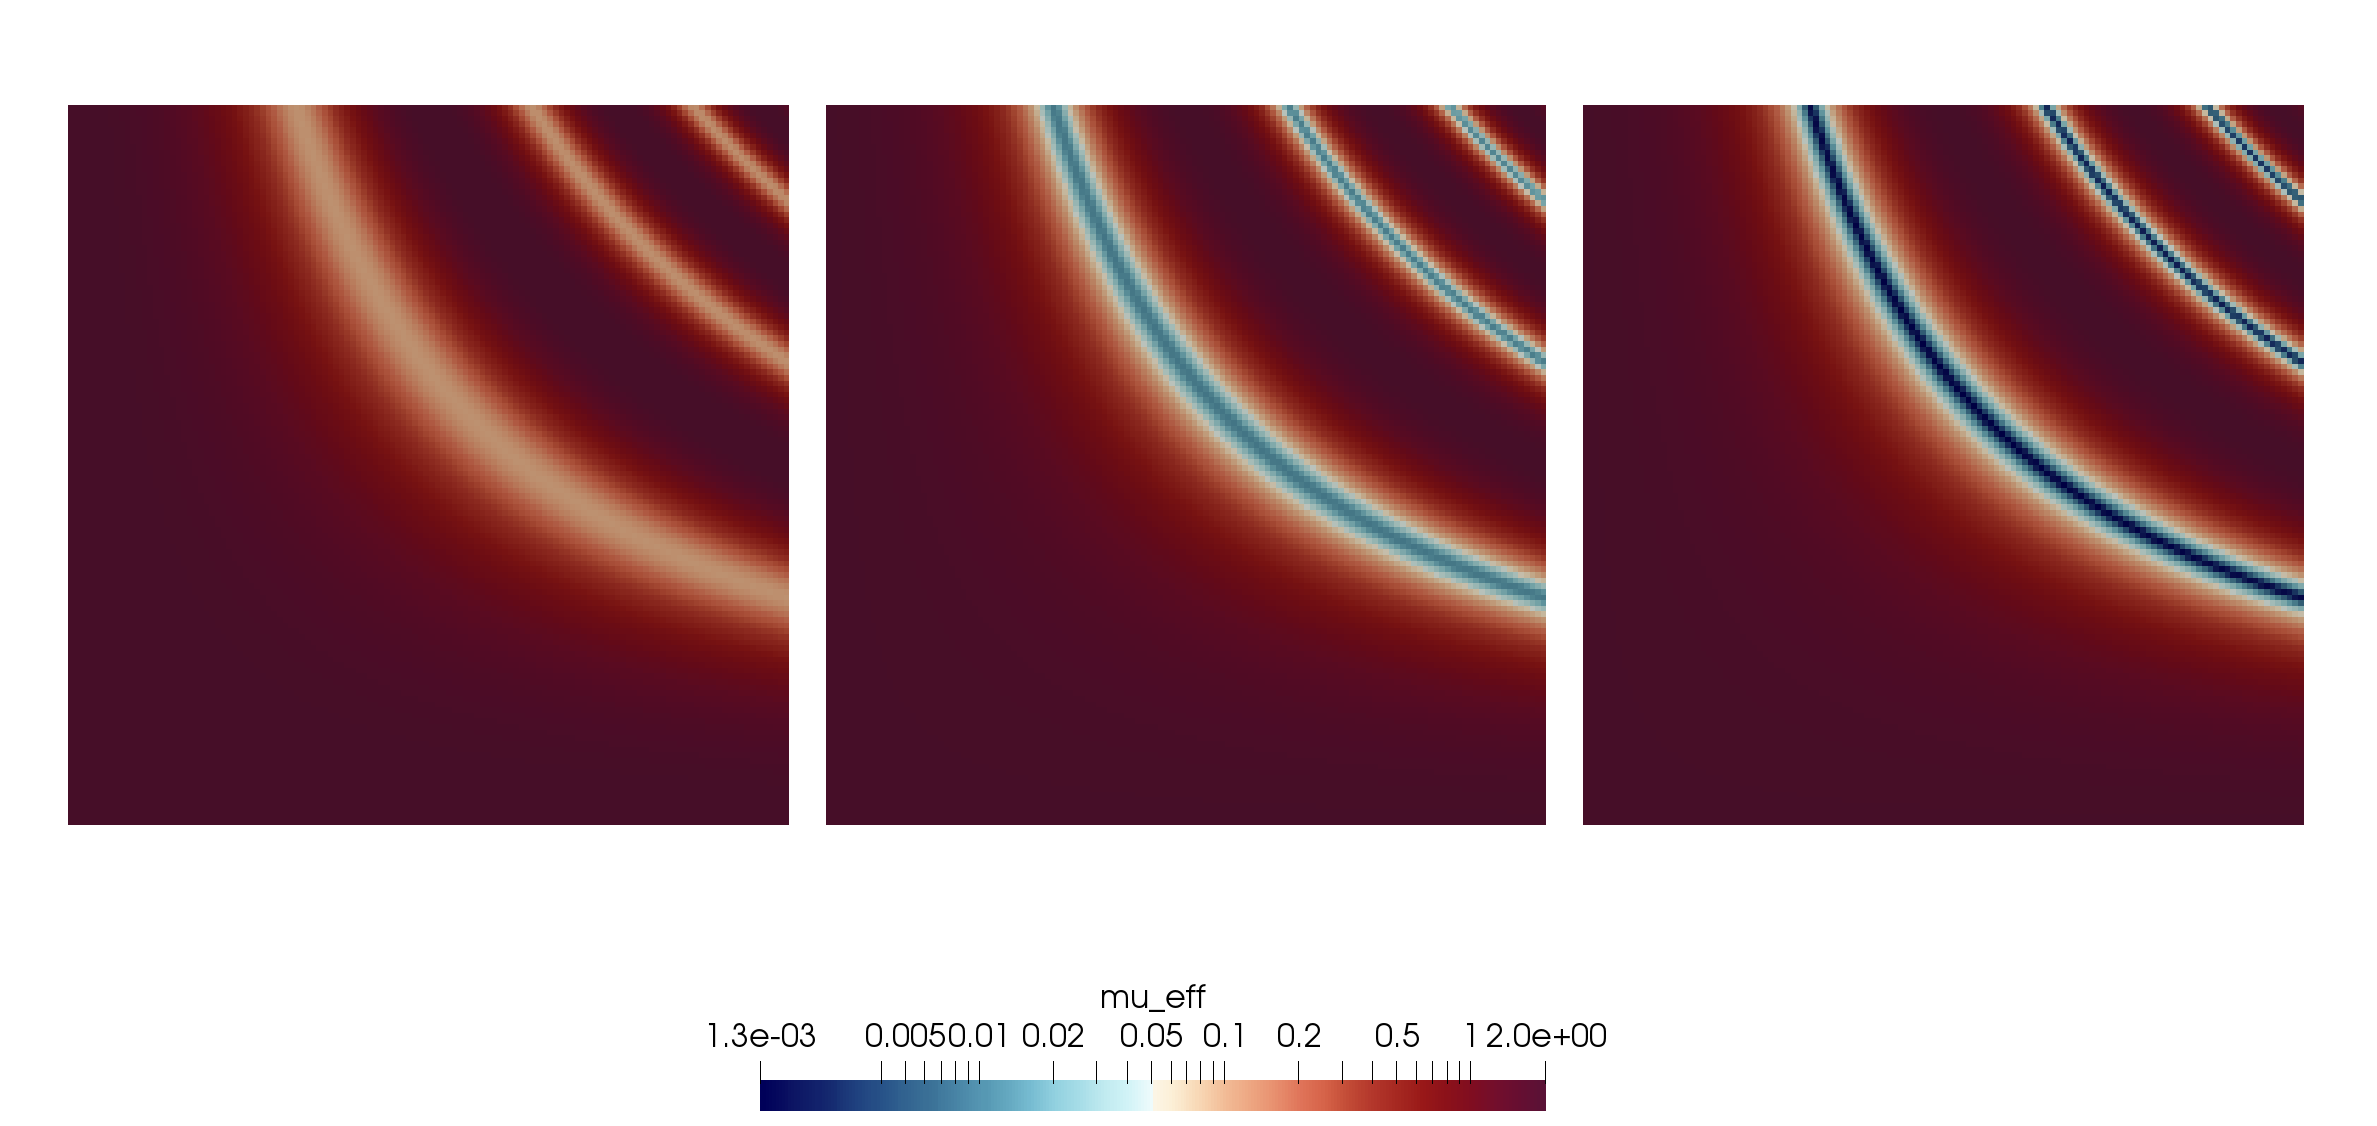
\includegraphics[width=14cm]{images/mms/mms7_mueffs}\\
Domain size 2x2 with $\epsilon=0.1, 0.01, 0.001$
\end{center}

Another interesting aspect of this benchmark is the fact that increasing the domain size
adds complexity to it as it increases the number of low viscosity zones and the spacing 
between them also decreases:

\begin{center}
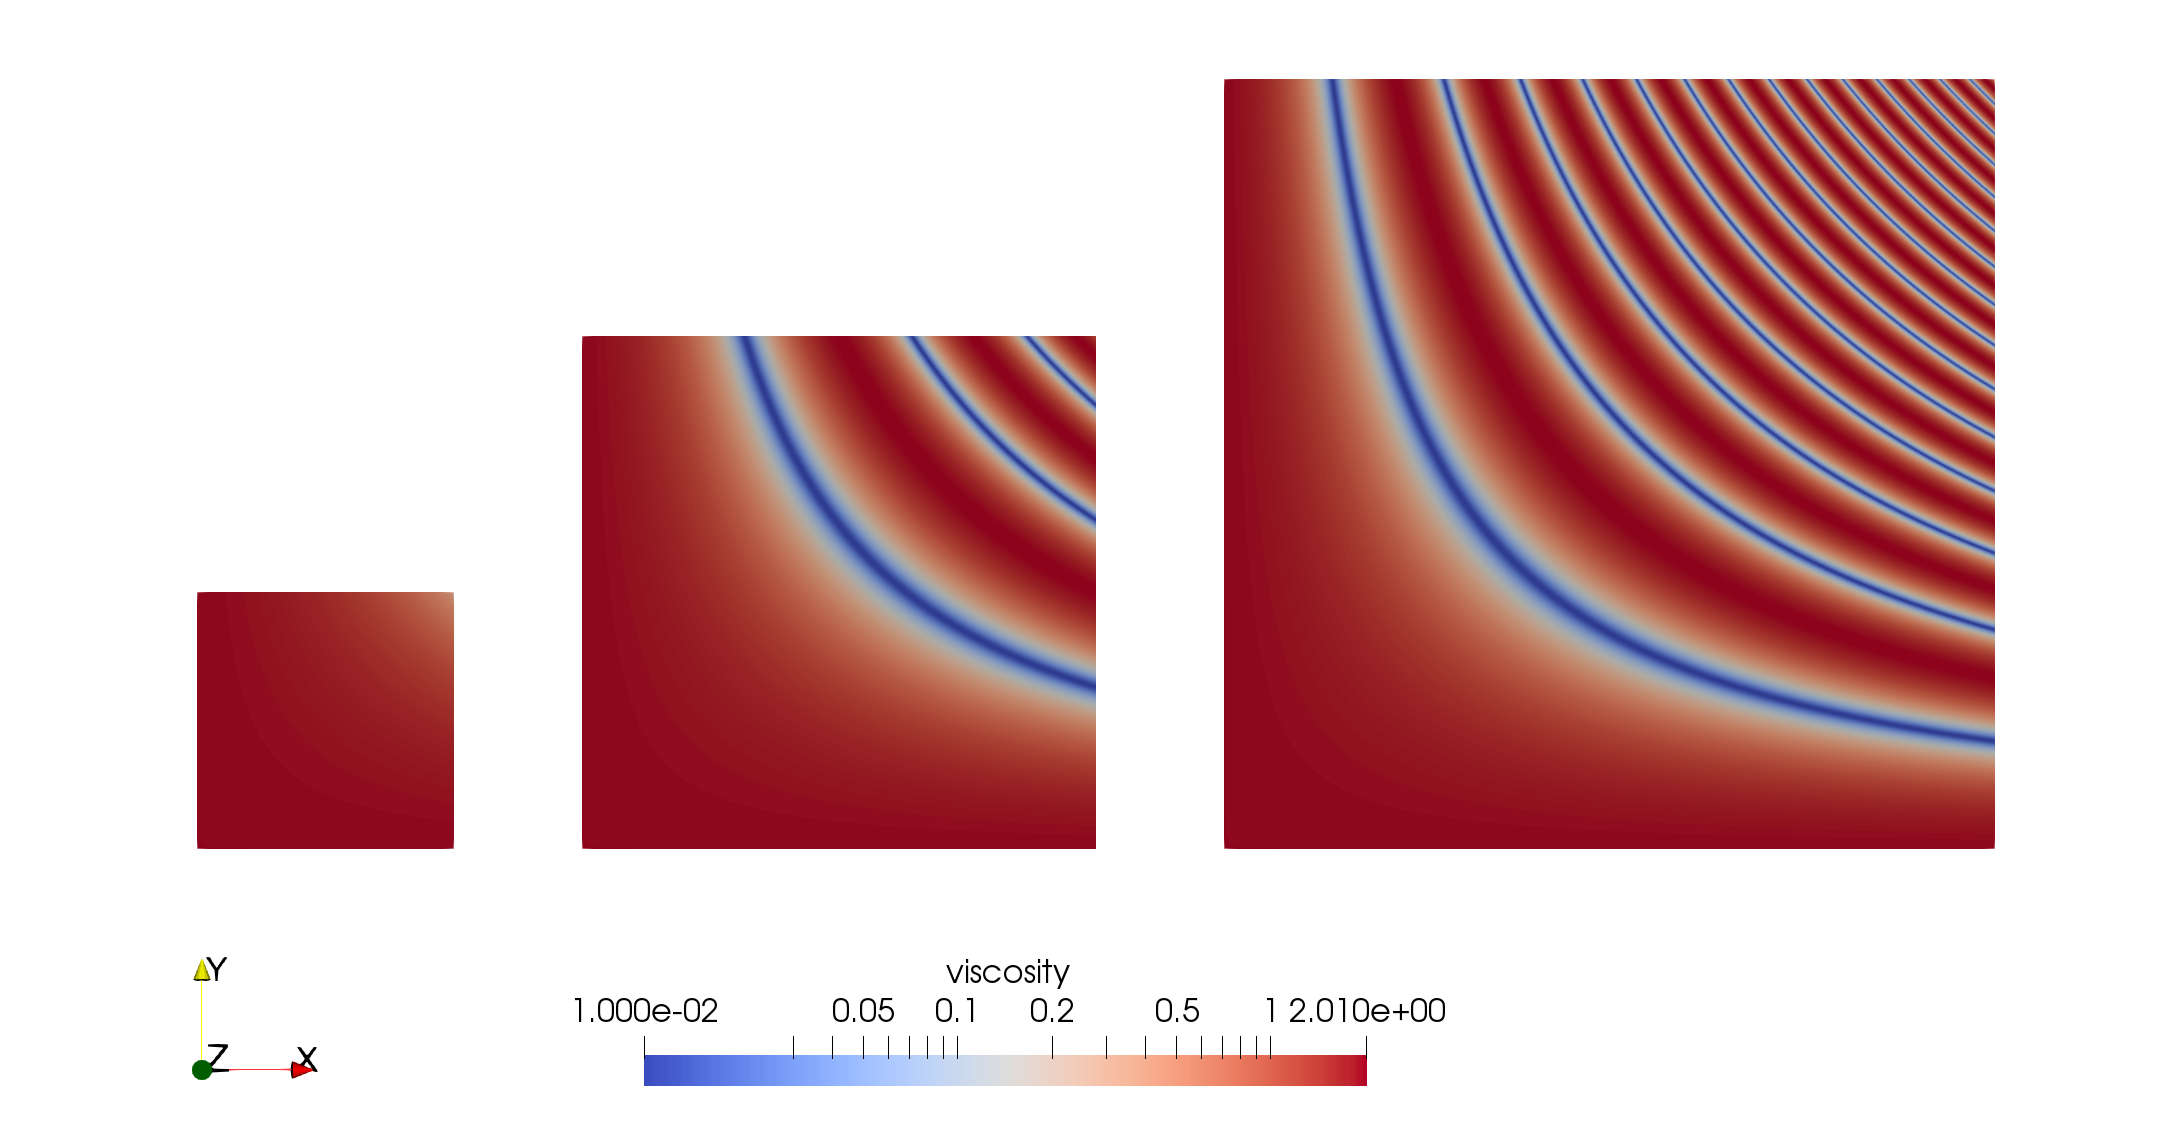
\includegraphics[width=7.28cm]{images/mms/mms7_visc}
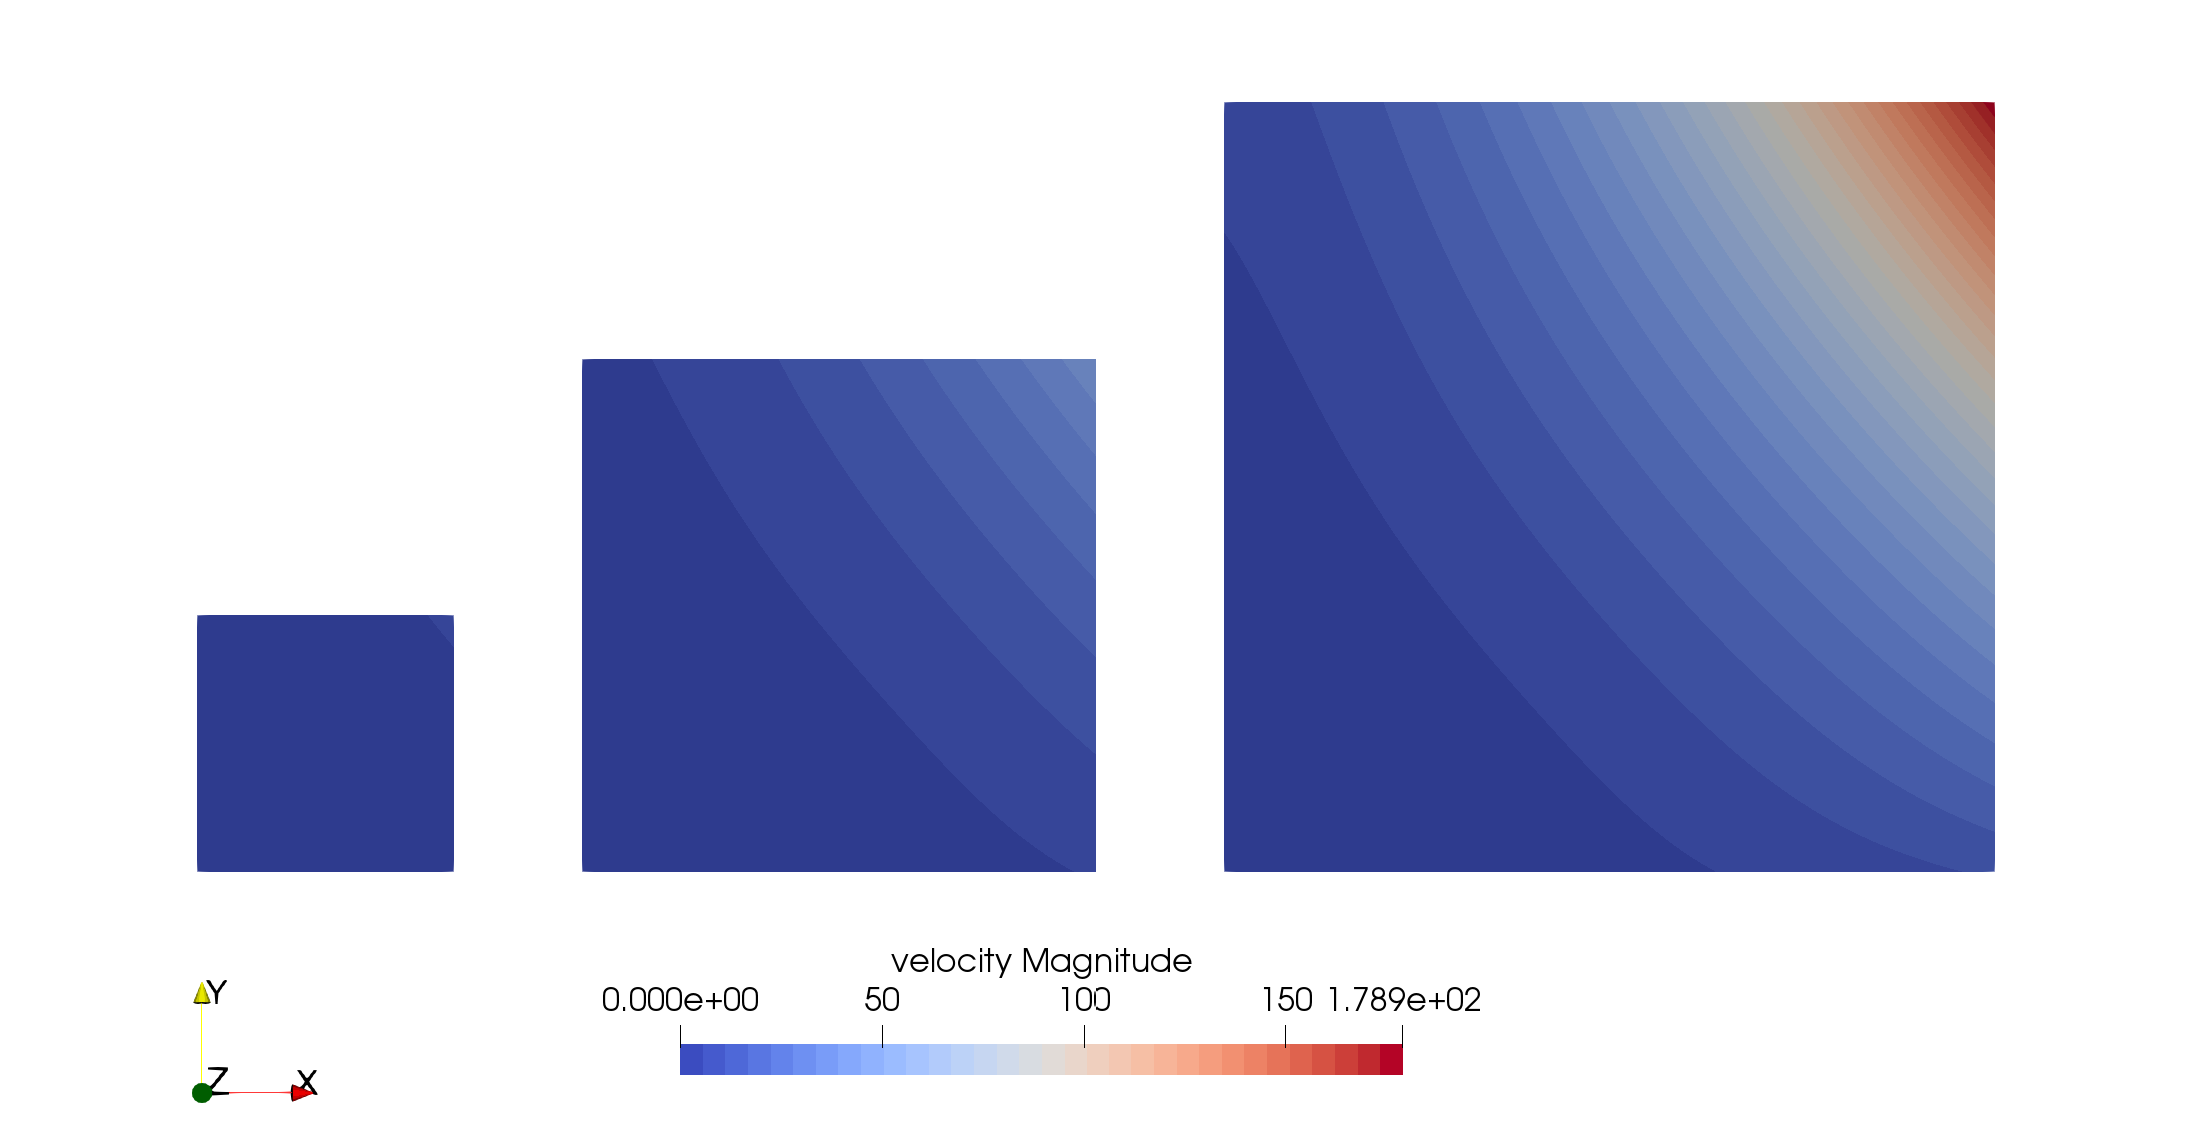
\includegraphics[width=7.28cm]{images/mms/mms7_vel}\\
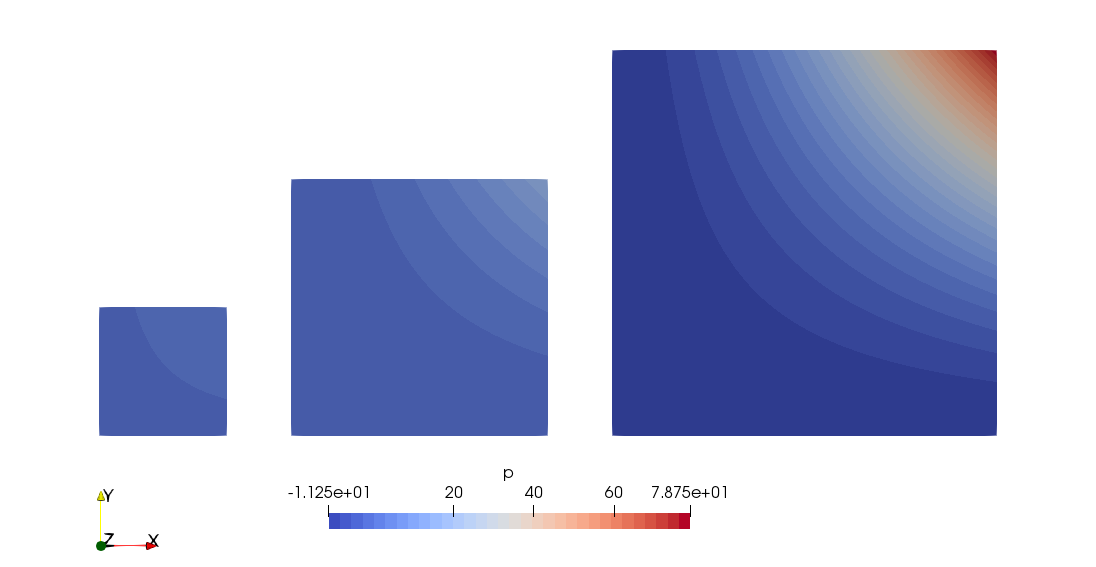
\includegraphics[width=7.28cm]{images/mms/mms7_press}
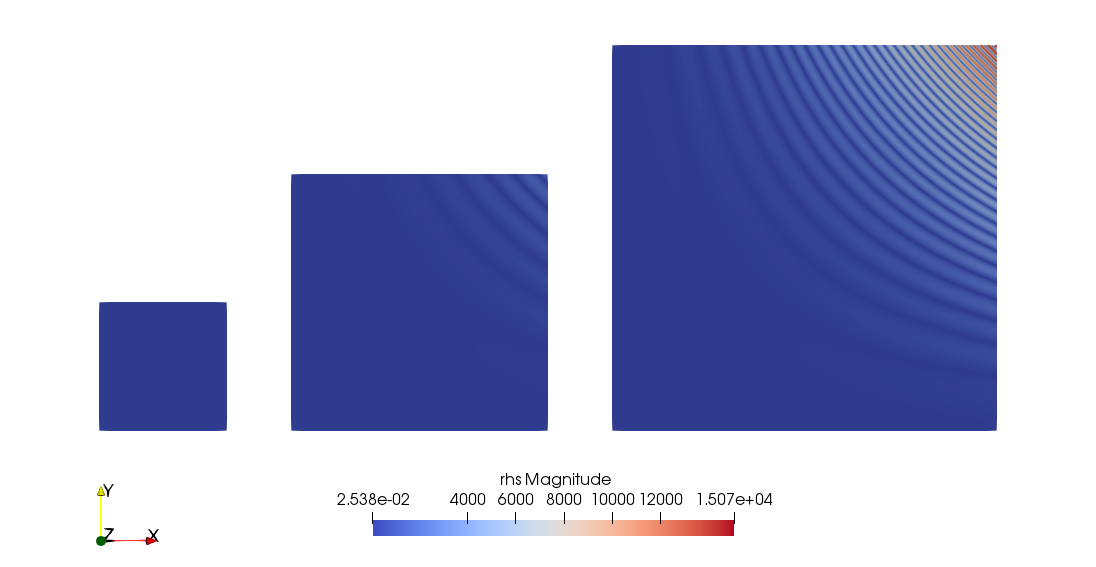
\includegraphics[width=7.28cm]{images/mms/mms7_rhs}\\
Three different domain sizes (1x1, 2x2, 3x3) with $\epsilon=0.001$.
\end{center}


Finally, because the analytical expression for both components of the velocity is a polynomial, we can also
compute the root mean square velocity exactly. For instance, for a 2x2 domain:
\begin{center}
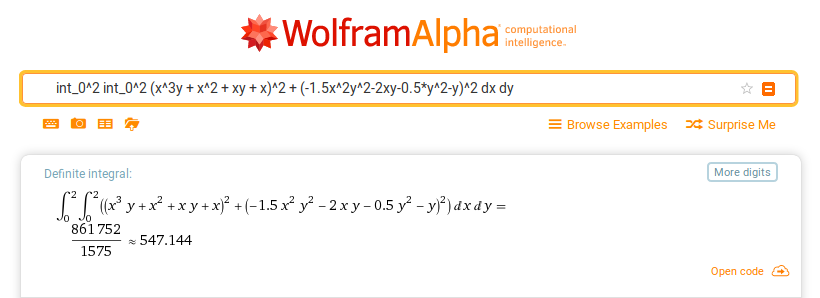
\includegraphics[width=8cm]{images/mms/mms7_vrmstheo}
\end{center}
and we end up with (for $L=2$)
\[
v_{rms} = \sqrt{\frac{1}{L^2}\frac{861752}{1575}} = \sqrt{\frac{215438}{1575}}
\simeq 11.6955560683
\]

\bscthesis \index{BSc Thesis}

%-----------------------------------------------------------------------------
\subsubsection{Analytical benchmark VIII \label{mms8} - "Kovasznay"}

This flow was published by L.I.G. Kovasznay in 1948 \cite{kova48}. 
This paper presents an exact two-dimensional solution of the Navier-Stokes equations 
with a periodicity in the vertical direction, 
gives an analytical solution to the steady-state Navier-Stokes equations that is similar
which is a flow-field behind a periodic array of cylinders.

\[
u(x,y)=1-\exp(\lambda x) \cos (2\pi y)
\qquad
\qquad
v(x,y)=\frac{\lambda}{2\pi} \exp(\lambda x) \sin (2 \pi y)
\qquad
\qquad
\lambda=\frac{Re}{2}-\sqrt{\frac{Re^2}{4}+4\pi^2}
\]

Following step-55 of deal.II \footnote{\url{https://www.dealii.org/current/doxygen/deal.II/step_55.html}}
we have to 'cheat' here since we are not solving the non-linear Navier-Stokes equations, but the linear Stokes system without convective term. Therefore, to recreate the exact same solution
we move the convective term into the right-hand side.

The analytical solution is prescribed left and right, while free/no (??) slip is prescribed at top and bottom.

Solution as implemented in step-55:
\begin{verbatim}
const double pi2 = pi*pi;
  u = -exp(x*(-sqrt(25.0 + 4*pi2) + 5.0))*cos(2*y*pi) + 1;
  v = (1.0L/2.0L)*(-sqrt(25.0 + 4*pi2) + 5.0)*exp(x*(-sqrt(25.0 + 4*pi2) + 5.0))*sin(2*y*pi)/pi;
  p = -1.0L/2.0L*exp(x*(-2*sqrt(25.0 + 4*pi2) + 10.0)) 
- 2.0*(-6538034.74494422 + 0.0134758939981709*exp(4*sqrt(25.0 + 4*pi2)))/(-80.0*exp(3*sqrt(25.0 + 4*pi2)) 
+ 16.0*sqrt(25.0 + 4*pi2)*exp(3*sqrt(25.0 + 4*pi2))) 
- 1634508.68623606*exp(-3.0*sqrt(25.0 + 4*pi2))/(-10.0 + 2.0*sqrt(25.0 + 4*pi2)) 
+ (-0.00673794699908547*exp(sqrt(25.0 + 4*pi2)) 
+ 3269017.37247211*exp(-3*sqrt(25.0 + 4*pi2)))/(-8*sqrt(25.0 + 4*pi2) + 40.0) 
+ 0.00336897349954273*exp(1.0*sqrt(25.0 + 4*pi2))/(-10.0 + 2.0*sqrt(25.0 + 4*pi2));
\end{verbatim}


%-----------------------------------------------------------------------------
\subsubsection{Analytical benchmark IX \label{mms9} - "VJ2"}

It is presented in \cite{jolm17} and meant to be a peculiar case where the velocity solution 
is exactly zero. The viscosity is 1, the domain is a unit square, no-slip boundary conditions 
are prescribed everywhere. The buoyancy force is given by $\vec{b}=(0,Ra(1-y+3y^2))$ where 
$Ra>0$ is a parameter. The flow is incompressible and the analytical pressure solution 
is given by $p=Ra(y^3-y^2/2+y-7/12)$.

%-----------------------------------------------------------------------------
\subsubsection{Analytical benchmark X \label{mms10} - "VJ3"}

This benchmark comes from John et al. \cite{jolm17}.
The domain is once again the unit square. The velocity field has the form of a large vortex.

\begin{eqnarray}
u(x,y) &=& 200x^2(1-x)^2y(1-y)(1-2y) \\
v(x,y) &=& -200x(1-x)(1-2x)y^2(1-y)^2 \\
p(x,y) &=& 10\left[(x-1/2)^3y^2+(1-x)^3(y-1/2)^3 \right]
\end{eqnarray}

\begin{center}
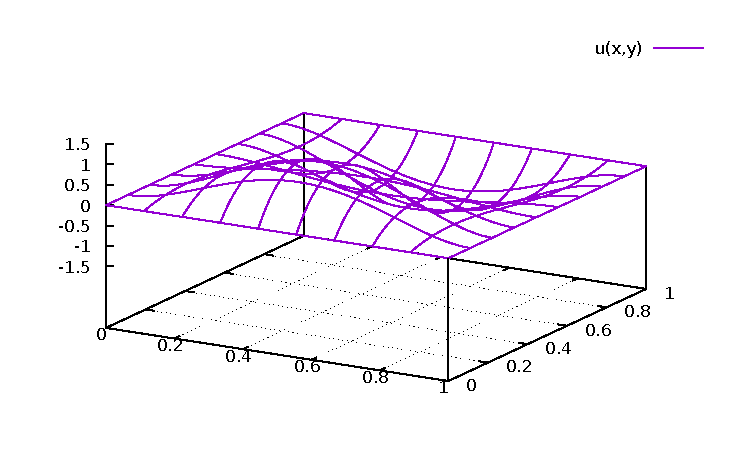
\includegraphics[width=4.5cm]{images/benchmark_VJ3/u.pdf}
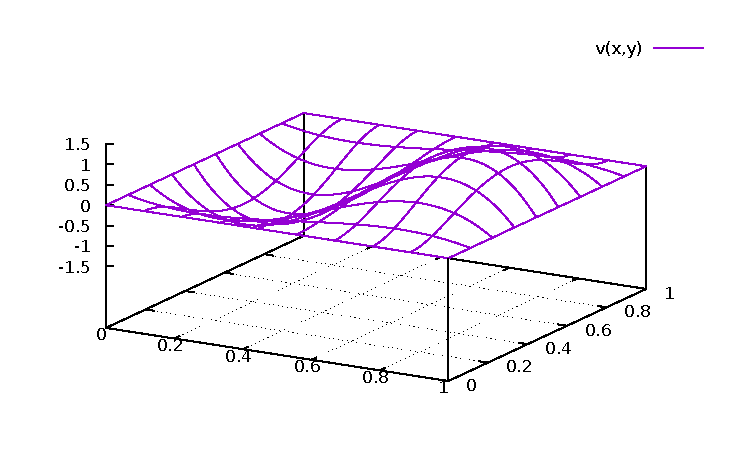
\includegraphics[width=4.5cm]{images/benchmark_VJ3/v.pdf}
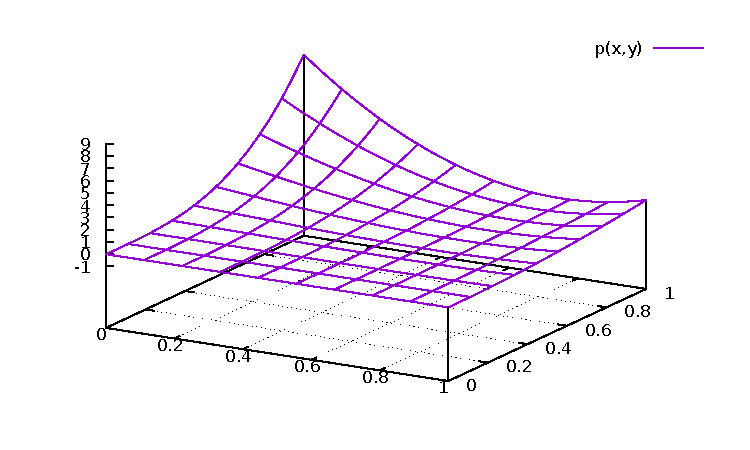
\includegraphics[width=4.5cm]{images/benchmark_VJ3/p.pdf}
\end{center}

\begin{eqnarray}
\dot{\varepsilon}_{xx}=\frac{\partial u}{\partial x} &=& -400(1-x)x(2x-1)(y-1)y(2y-1)  \\
\frac{\partial u}{\partial y} &=& 200(1-x)^2x^2 (6y^2-6y+1)  \\
\frac{\partial v}{\partial x} &=& -200(6x^2-6x+1)(1-y)^2y^2  \\
\dot{\varepsilon}_{yy}=\frac{\partial v}{\partial y} &=& 400(x-1)x(2x-1)(1-y)y(2y-1) 
\end{eqnarray}
so that 
\begin{eqnarray}
\dot{\varepsilon}_{xy}
&=&\frac{1}{2} \left[ 200(1-x)^2x^2 (6y^2-6y+1)   -200(6x^2-6x+1)(1-y)^2y^2  \right] \nn\\
&=&100(1-x)^2x^2 (6y^2-6y+1)   -100(6x^2-6x+1)(1-y)^2y^2 
\end{eqnarray}
Also
\begin{eqnarray}
\frac{\partial \dot{\varepsilon}_{xx}}{\partial x} &=& 400(6x^2-6x+1)y(2y^2-3y+1) \nn\\
\frac{\partial \dot{\varepsilon}_{xy}}{\partial x} 
&=& 200 (-2 x^2 (1 - x) (6 y^2 - 6 y + 1) + 2 x (1 - x)^2 (6 y^2 - 6 y + 1) - 6 (2 x - 1) (1 - y)^2 y^2)\nn\\
&=&  100 (-2 x^2 (1 - x) (6 y^2 - 6 y + 1) + 2 x (1 - x)^2 (6 y^2 - 6 y + 1) - 6 (2 x - 1) (1 - y)^2 y^2) \nn\\
\frac{\partial \dot{\varepsilon}_{xy}}{\partial y} &=& 400 (6 x^2 - 6 x + 1) (1 - y) y^2 + 200 (1 - x)^2 x^2 (12 y - 6) - 400 (6 x^2 - 6 x + 1) (1 - y)^2 y   \nn \\
\frac{\partial \dot{\varepsilon}_{yy}}{\partial y} &=& -400x(2x^2-3x+1)(6y^2-6y+1) 
\end{eqnarray}


\begin{eqnarray}
\frac{\partial p}{\partial x} &=& 30(x-1/2)^2y^2-30(1-x)^2(y-1/2)^3 \\
\frac{\partial p}{\partial y} &=& 20(x-1/2)^3y + 30(1-x)^3(y-1/2)^2  
\end{eqnarray}

From $\vec\nabla\cdot{\bm \sigma}+\vec{b}=\vec{0}$ we can obtain the rhs as follows:
\begin{eqnarray}
\vec{b} 
&=& - \vec\nabla\cdot{\bm \sigma} \nn\\ 
&=& \vec\nabla p -  \vec\nabla\cdot{\bm s} \nn\\ 
&=& \vec\nabla p -  \vec\nabla\cdot(2 \eta \dot{\bm \varepsilon})  
\end{eqnarray}
Assuming $\eta=1$ we arrive at:
\begin{eqnarray}
b_x &=&  \frac{\partial p}{\partial x} 
-2\frac{\partial \dot{\varepsilon}_{xx}}{\partial x}  
-2\frac{\partial \dot{\varepsilon}_{xy}}{\partial y}  \\
b_y &=&  \frac{\partial p}{\partial y}  
-2\frac{\partial \dot{\varepsilon}_{xy}}{\partial x} 
-2\frac{\partial \dot{\varepsilon}_{yy}}{\partial y}  
\end{eqnarray}

All the necessary functions to do this benchmark are in {\tt mms/vj3.py}:
\lstinputlisting[language=python]{mms/vj3.py}

\begin{center}
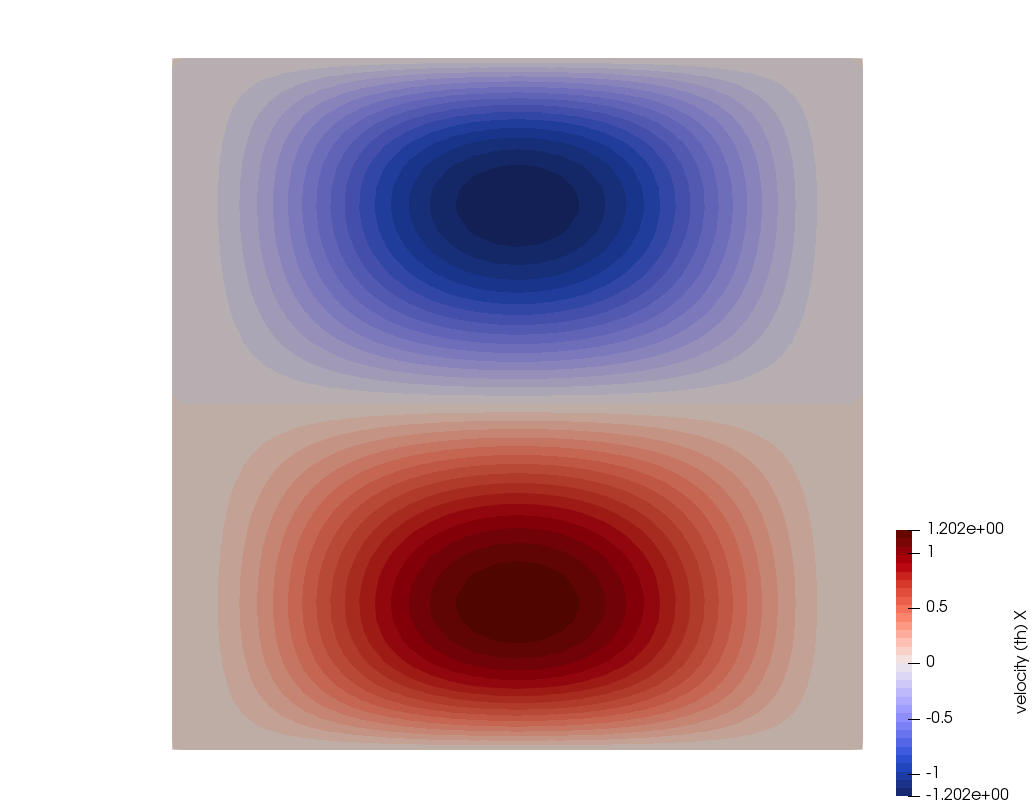
\includegraphics[width=4.5cm]{images/mms/vj3/u}
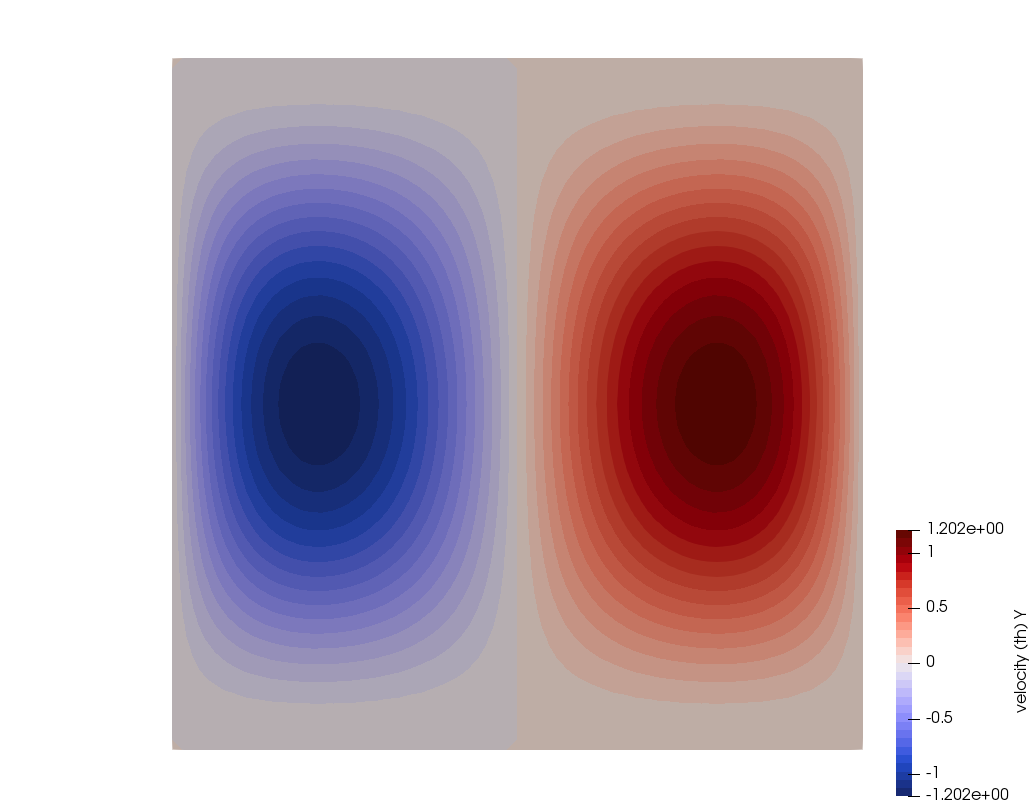
\includegraphics[width=4.5cm]{images/mms/vj3/v}
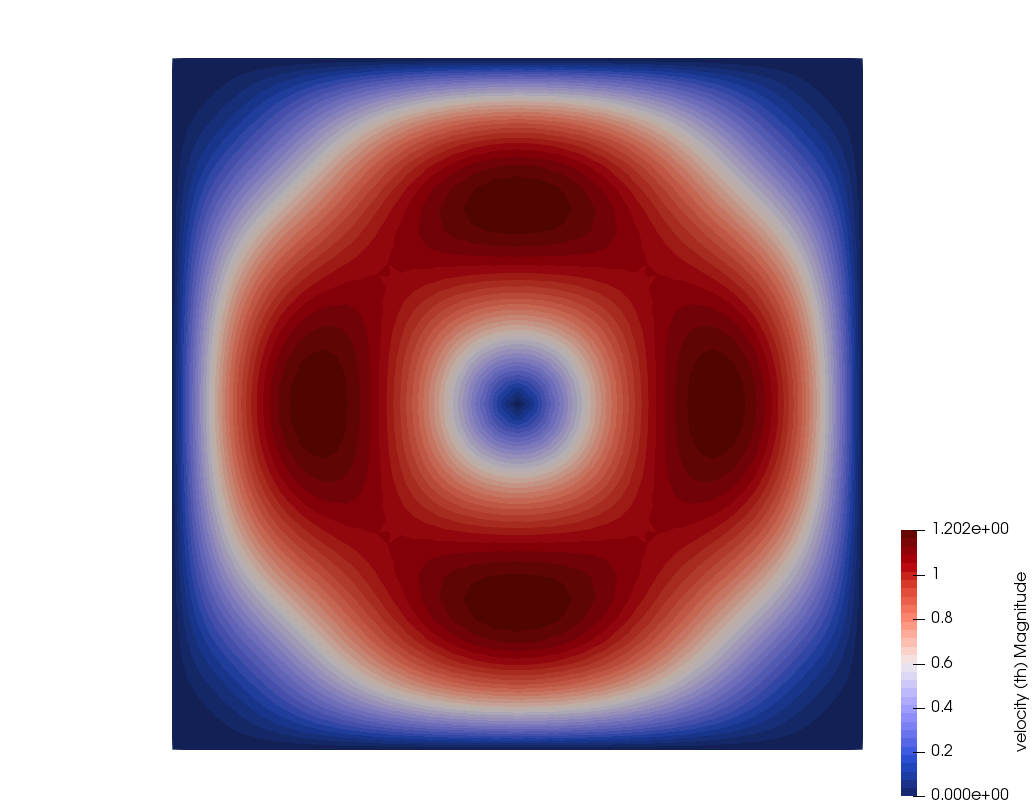
\includegraphics[width=4.5cm]{images/mms/vj3/vel}\\
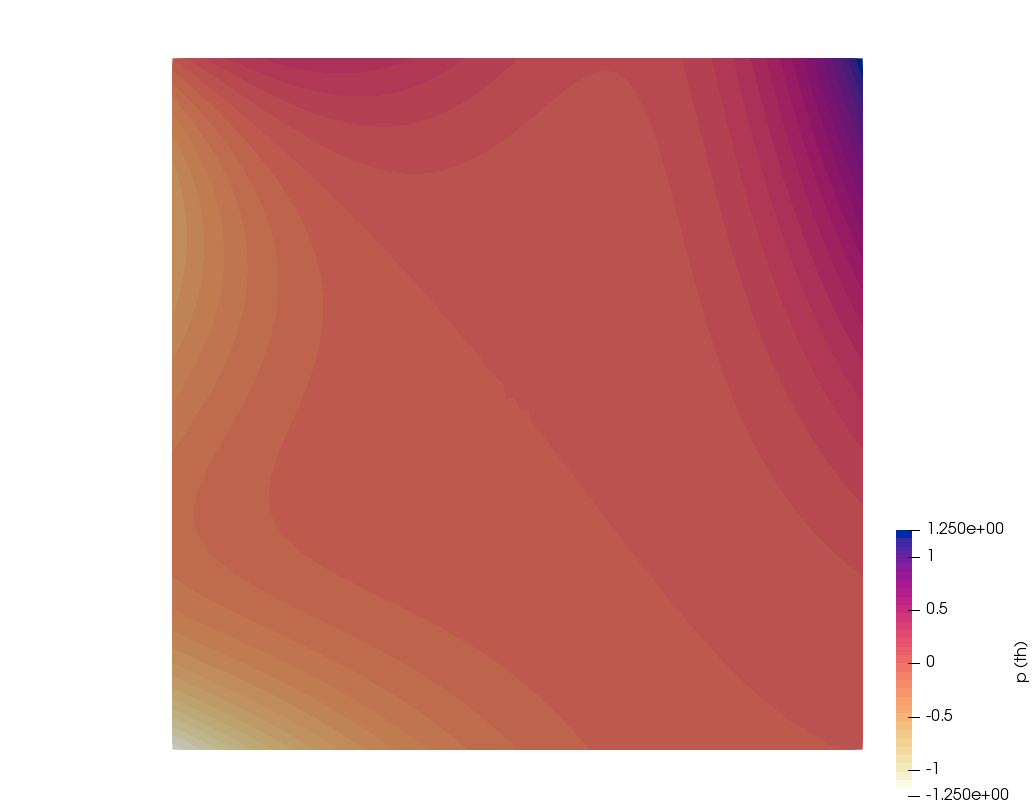
\includegraphics[width=4.5cm]{images/mms/vj3/p}
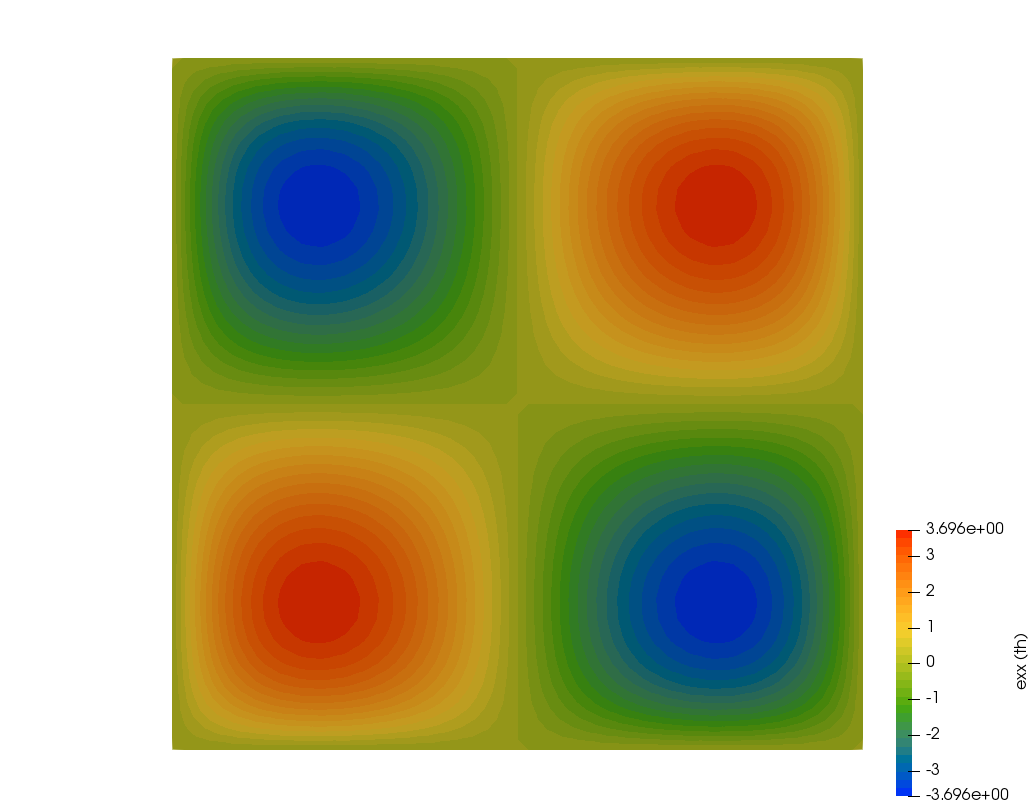
\includegraphics[width=4.5cm]{images/mms/vj3/exx}
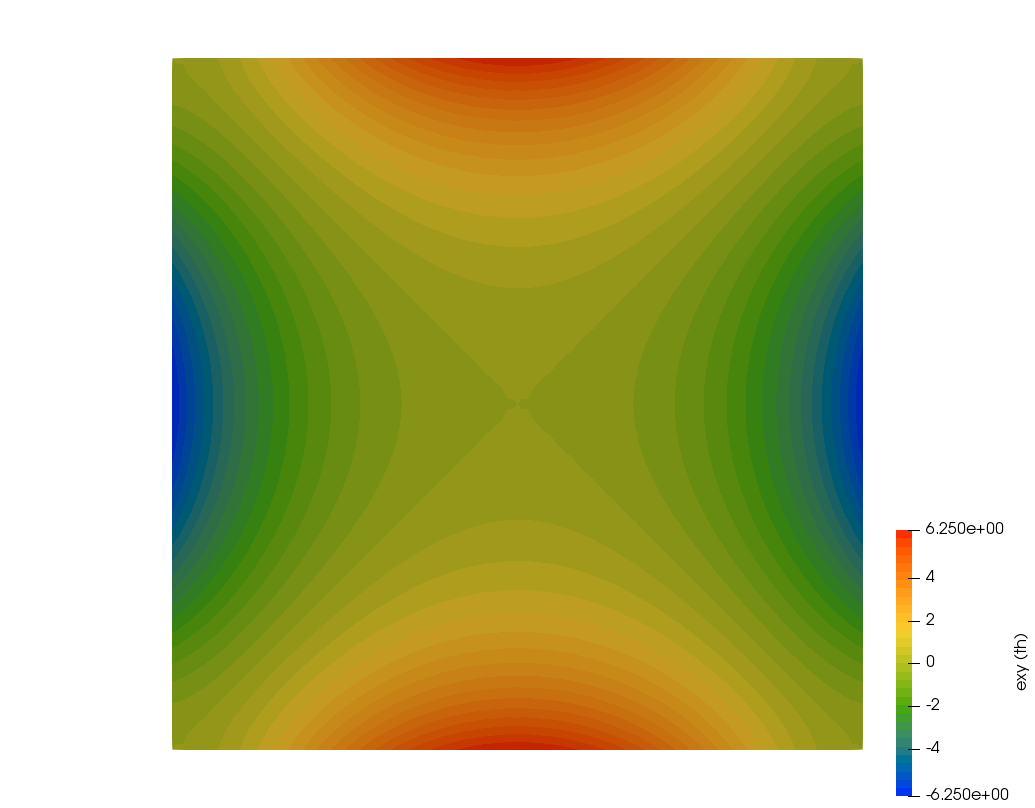
\includegraphics[width=4.5cm]{images/mms/vj3/exy}
\end{center}

%-----------------------------------------------------------------------------
\subsubsection{Analytical benchmark XI \label{mms11} - "PPC1"}



%-----------------------------------------------------------------------------
\subsubsection{Analytical benchmark XII \label{mms11} - "PPC2"}





